\section{State regulator}
General assumptions: the plant is controllable and observable.
The plant is a \emph{low-pass} system and $D=0$.

\subsection{State Feedback}

\begin{minipage}{10cm}
    The whole system can be described by
    \begin{align*}
        A_g &= A-BK & B_g &= B K_{vf} & C_g &= C
    \end{align*}
    and
    \[
        G(s) = \frac{Y(s)}{R(s)} = C(sI-A+BK)^{-1}BK_{vf}
    \]
    where
    \[
        K_{vf} = (C(-A+BK)^{-1}B)^{-1}
    \]
\end{minipage}
\hspace{0.5cm}
\begin{minipage}{8cm}
    \centering
    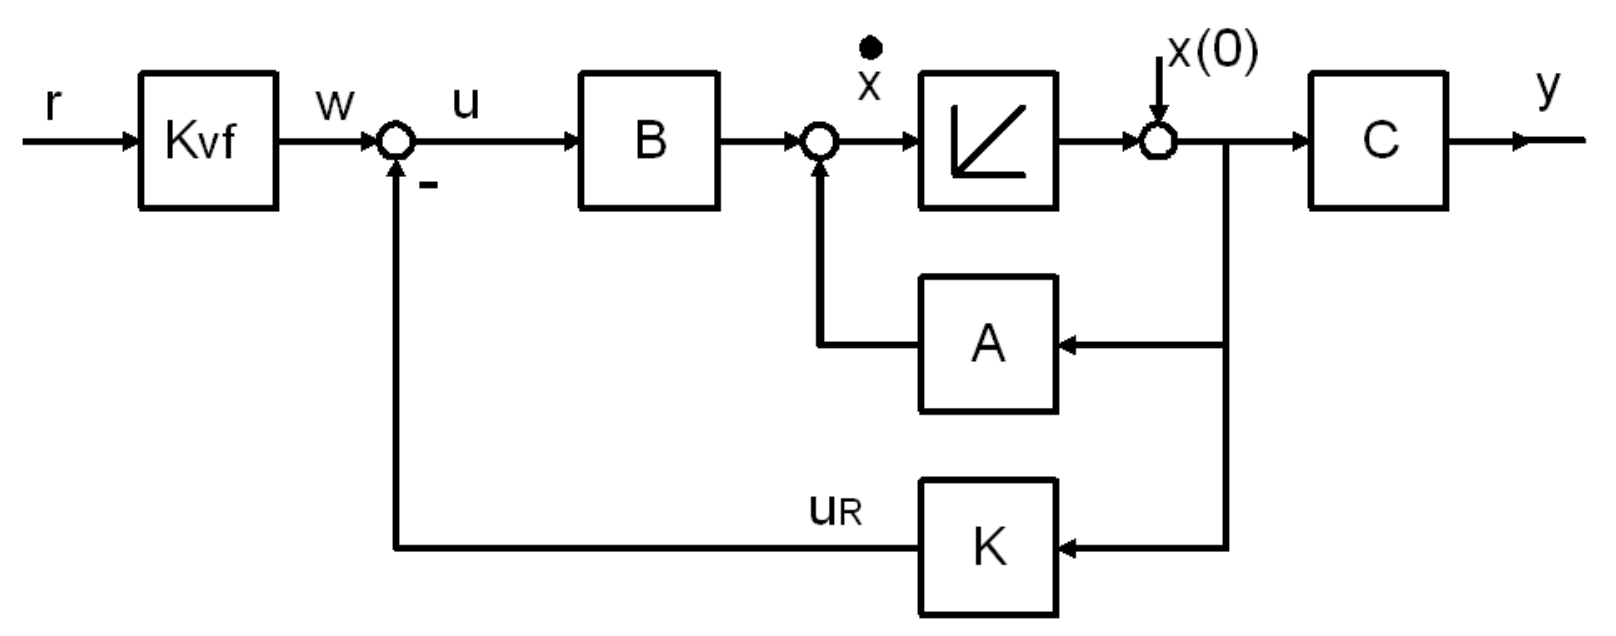
\includegraphics[width=\linewidth]{./bilder/statereg.png}
\end{minipage}

\subsection{Pole Placement}
\begin{minipage}{10cm}
Controllability ensures that the eigenvalues of $A_g$ can be placed arbitrarily by choice of $K$
To achieve some desired eigenvalues, the following must hold:
\[
    \det(\lambda I-A+BK) = (\lambda - \lambda_1)...(\lambda - \lambda_n)
\]
Some considerations:
\begin{itemize}
    \item Only left half plane (stability)
    \item Transients should decay faster than some $C \cdot e^{-\sigma_1}$
    \item Transients should be well damped: $\zeta > \frac{1}{\sqrt{2}}$
    \item Upper bound to save energy $\sigma < \sigma_2$
\end{itemize}

\end{minipage}
\hspace{0.5cm}
\begin{minipage}{8cm}
    \centering
    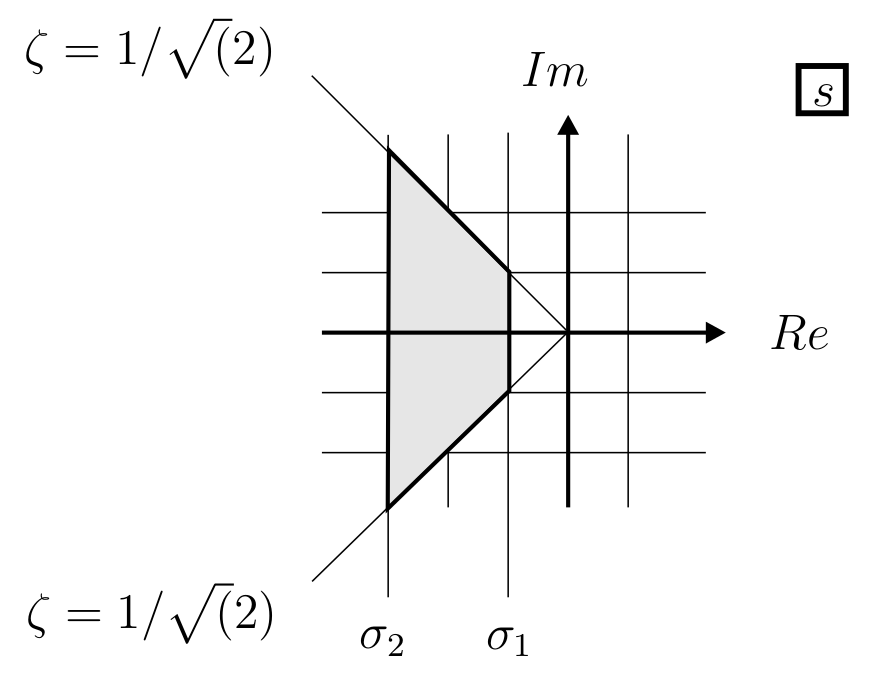
\includegraphics[width=5cm]{./bilder/pole_locations.png}
\end{minipage}

\subsection{Optimal control}
General consideration: minimize a cost function (performance index) $J = f(K)$.
General notation:
\[
    J = f(K) = \int_{0}^{t_f} g(x,u) dt
\]
We define $H = A - BK$ and introduce a positive semidefinite weighting matrix $Q$.
To minimize the norm of the state variable $x$: $|x|^2 = x^Tx$, we get:
\begin{align*}
    J &= \int_0^{\infty} x^T Q x \, dt = x^T(0) P x(0) & \text{and} && (H^TP + PH) &= -Q
\end{align*}

Design steps:
\begin{enumerate}
    \item Determine the matrix $P$, where $H$ and $Q$ are assumed to be known.
    \item Minimize $J = x^T(0) P x(0)$ by adjusting system parameters.
\end{enumerate}

\subsection{Linear Quadratic Regulator (LQR)}
To consider the control energy of $u$, the performance index becomes
\[
    J = \int_{0}^{\infty} (x^T Q x + u^T R u) dt
\]
where $Q$ and $R$ are positive definite.
$J$ is minimized with
\[
    K = R^{-1} B^T P
\]
$P$ is calculated with the algebraic matrix Riccati (ARE), which is a quadratic equation.
Only the positive definite solution of $P$ is valid.
\[
    A^T P + P A - P B R^{-1} B^T P = -Q
\]

Design steps:
\begin{enumerate}
    \item Determine $P$, where $Q$ and $R$ have to be known (often $I$).
    \item Calculate $K = R^{-1} B^T P$
\end{enumerate}

\paragraph{Robustness}If the control loop is opened at the input $u$, the open
loop transfer function becomes $G_0(s) = K (sI-A)^{-1} B$.
This fulfills the \emph{Kalman inequality} $|1+G_0(j\omega)|\geq 1$.
From this a phase margin of $\pm 60^{\circ}$ and a gain margin $>0.5$ can be
calculated.
This makes LQR a very robust controller.

\subsection{State Regulator with Integral Part}
\begin{minipage}{10cm}
    A regulator with $K_1$ containing an integral part can be designed by
    viewing $K_1$ and $K_2$ as cascaded controllers.
    The controller can then be designed in two steps: a faster inner loop (e.g. LQR)
    and a slower outer loop (often PI-controller).
    
    To calculate $K_1$ and $K_2$ at once, one defines the error $e = y-r$ and the
    intermediate variables $z = \dot{x}$ and $w=\dot{u}$. Then:
    \[
        \underbrace{\begin{bmatrix}
        \dot{e} \\ \dot{z}
        \end{bmatrix}}_{\dot{\hat{x}}}
      = \underbrace{\begin{bmatrix}
            0 & C \\ 0 & A
        \end{bmatrix}}_{\hat{A}}
        \underbrace{\begin{bmatrix}
            e \\ z
        \end{bmatrix}}_{\hat{x}}
      + \underbrace{\begin{bmatrix}
            0 \\ B
        \end{bmatrix}}_{\hat{B}}
        \underbrace{w}_{\hat{u}}
    \]
   
\end{minipage}
\hspace{0.5cm}
\begin{minipage}{8cm}
    \centering
    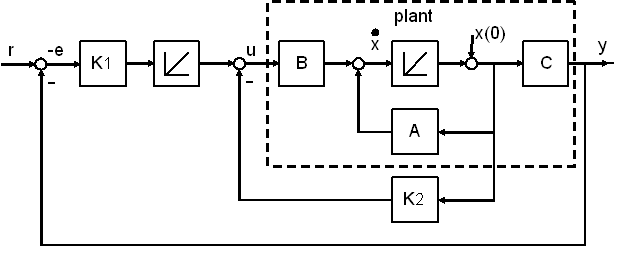
\includegraphics[width=8cm]{./bilder/statereg_int.png}
\end{minipage}

Now the feedback gain $\hat{K}$ which stabilizes this equation can be designed
e.g. by LQR or pole placement.

\subsection{State Regulator with Observer}
\begin{minipage}{10cm}
    If not all state variables are available for feedback, they can be reconstructed by modeling the plant
    using an observer: $\dot{\hat{x}} = A\hat{x} + Bu$.
    It follows that
    \[
        \dot{\hat{x}} = (A-HC) \hat{x} + Bu + HCx
    \]
    The observer can be calculated by LQR in a dual way by using the following correspondences:
    \begin{align*}
        \text{Regulator} &\Leftrightarrow \text{Observer} & \text{Regulator} &\Leftrightarrow \text{Observer} \\
        P_c &\Leftrightarrow P_o^T &
        B &\Leftrightarrow C^T \\
        A &\Leftrightarrow A^T &
        K &\Leftrightarrow H^T
    \end{align*}
    The calculation of the optimal $H$ is called the \emph{Linear Quadratic Gaussian (LQG)} problem and is
    \begin{enumerate}
        \item $AP + PA^T - PC^TR^{-1}CP = -Q$ which deliveres $P$
        \item $H = (R^{-1}CP)^T = PC^TR^{-1}$
    \end{enumerate}
    
\end{minipage}
\hspace{0.5cm}
\begin{minipage}{8cm}
    \centering
    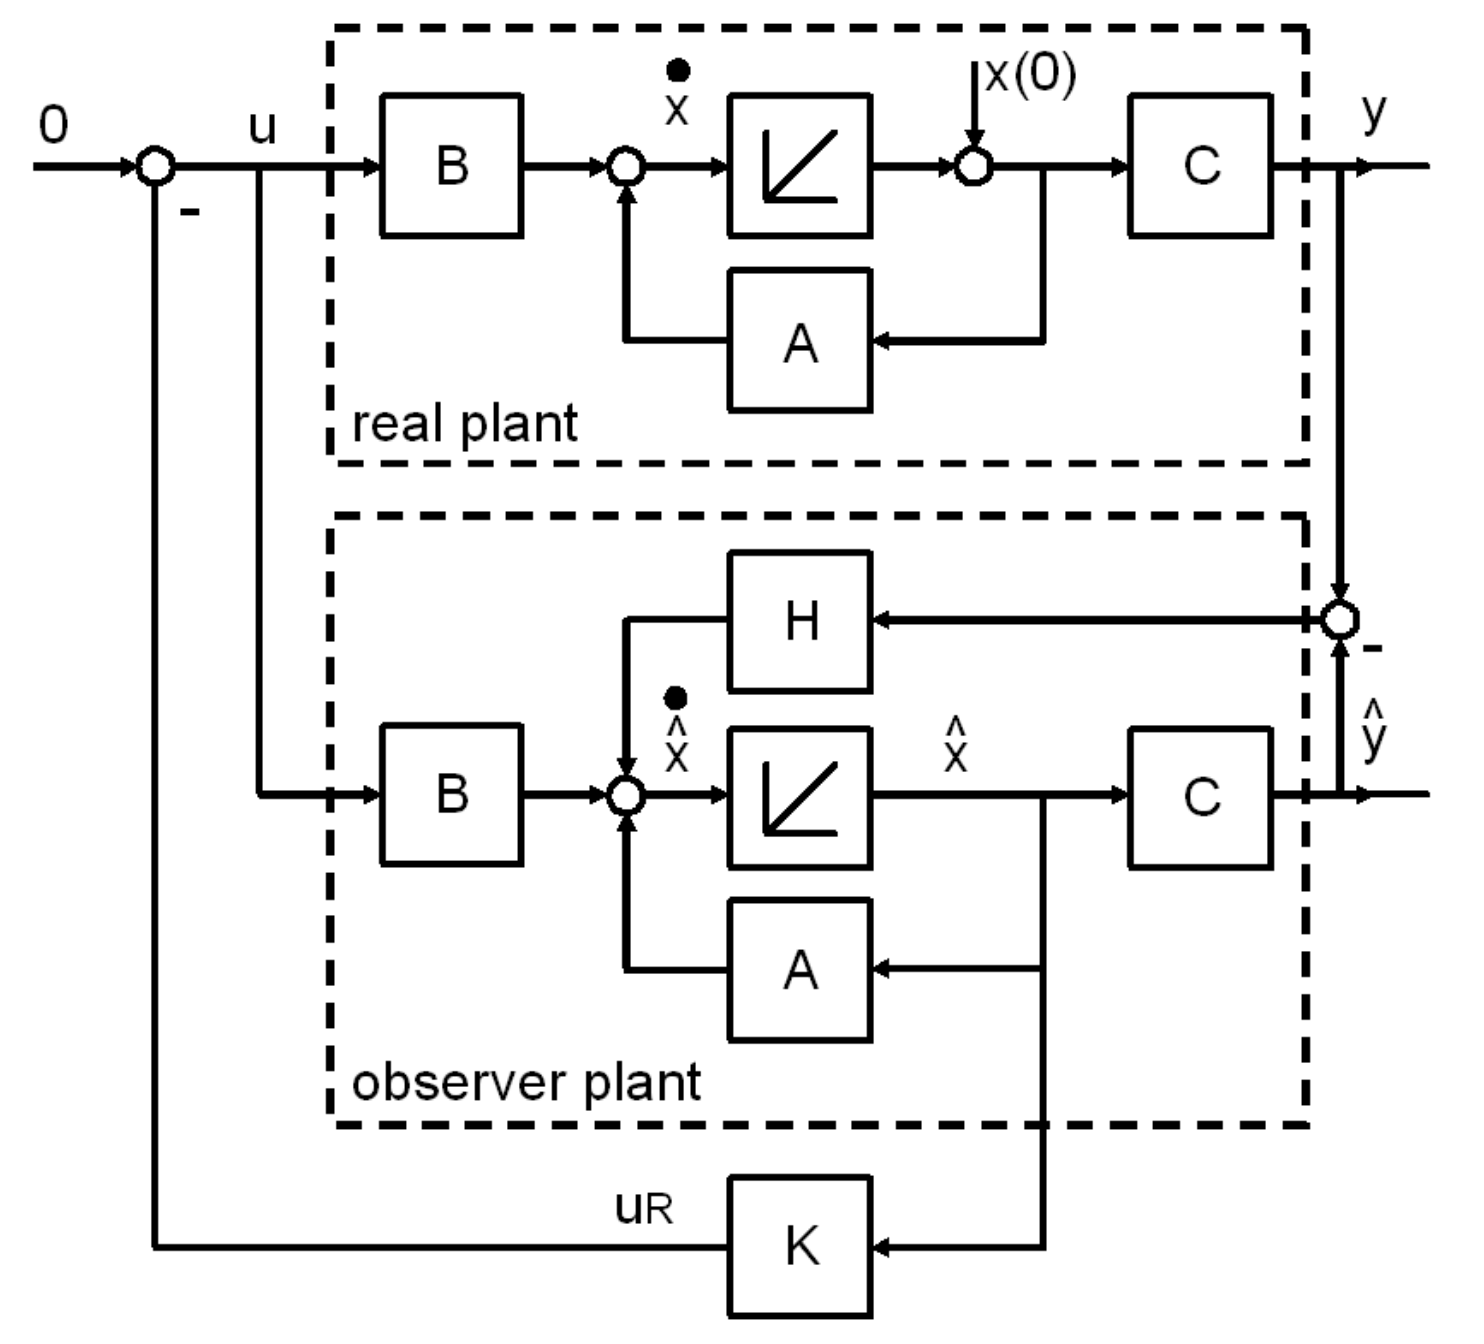
\includegraphics[width=7cm]{./bilder/observer.png}
\end{minipage}

\subsection{Combined LQR and LQG design}
The overall system is now given by
\[
    \begin{bmatrix}
        \dot{x} \\ \dot{\tilde{x}}\\
    \end{bmatrix} = 
    \begin{bmatrix}
        A-BK && BK \\
        0 && A-HC \\
    \end{bmatrix}
    \begin{bmatrix}
        x \\ \tilde{x} \\
    \end{bmatrix}
\]
The characteristic equation of this system is
\[
    \det\begin{bmatrix}
        sI - A + BK & -BK \\
        0 & sI - A + HC
    \end{bmatrix}
    =
    \det(sI - A + BK) \cdot \det(sI - A + HC) = 0
\]
It follows that the controller and the observer can be separated
and can thus be designed independently.

\vspace{1em}
\begin{minipage}{10cm}
    \paragraph{Compensator}Rearranging the block diagram, one can create
    a compensator block.
    The transfer function of the compensator is then
    \[
        G_c(s) = \frac{U(s)}{E(s)} = K(sI - A + BK + HC)^{-1} H
    \]
    or with the loop opened at the plant input $u$:
    \[
        G_0(s) = K(sI - A + BK + HC)^{-1} H \cdot C(sI - A)^{-1} B
    \]
\end{minipage}
\hspace{0.5cm}
\begin{minipage}{8cm}
    \centering
    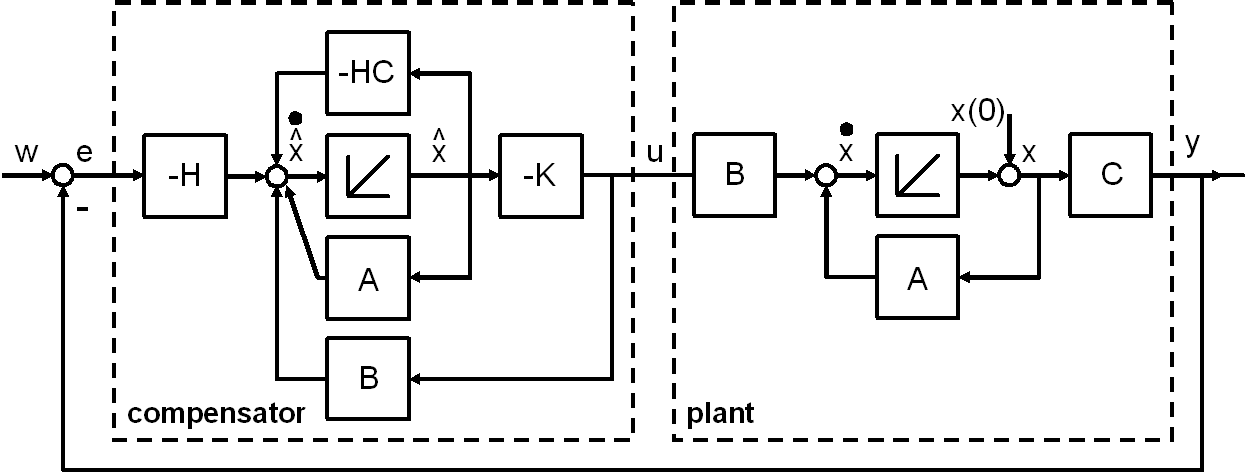
\includegraphics[width=8cm]{bilder/statereg_comp.png}
\end{minipage}

\vspace{0.5em}
Unlike $G_{0,reg}$ and $G_{0,obs}$, which have a phase margin of at least
$\pm 60^{\circ}$ a gain margin $>0.5$, the compensator does \emph{not} have
any guaranteed margin.

\subsection{Loop Transfer Recovery (LQG/LTR and LQR/LTR)}
If some robustness is required, the LQR and LQG designs cannot be carried out independently.
\begin{enumerate}
    \item Design LQR with arbitrary weighting matrices, resulting in a regulator gain $K$.
    \item Do LQG design with $Q = \rho B B^T$ and $R = I$, resulting in an observer gain $H$.
\end{enumerate}
Then, if $G(s)$ is minimum-phase,
\[
    \lim_{\rho\to\infty} G_0(s) = K(sI - A)^{-1} B = G_{0,reg}(s)
\]
which has a guaranteed gain and phase margins.

Similarly, due to duality, if the loop is opened at the output $y$, the transfer function
becomes
\[
    \hat{G}_0(s) = C(sI-A)^{-1} B \cdot K(sI - A + BK + HC)^{-1} H
\]
With $Q =\rho C^T C$ and $R=I$, the LQR design design recovers the LQG loop transfer function,
which leads to
\[
    \lim_{\rho\to\infty} = C(sI-A)^{-1}H = G_{0,obs}(s)
\]
which is called the dual LQG/LTR method.